% ------------------------------------------------------------------
\chapter{Introduction to MatConvNet}\label{s:intro}
% ------------------------------------------------------------------

\matconvnet is a MATLAB toolbox implementing \emph{Convolutional Neural Networks} (CNN) for computer vision applications.  Since the breakthrough work of~\cite{krizhevsky12imagenet}, CNNs have had a major impact in computer vision, and image understanding in particular, essentially replacing traditional image representations such as the ones implemented in our own VLFeat~\cite{vedaldi10vlfeat} open source library.

While most CNNs are  obtained by composing simple linear and non-linear filtering operations such as convolution and rectification, their implementation is far from trivial. The reason is that CNNs need to be learned from vast amounts of data, often millions of images, requiring very efficient implementations. As most CNN libraries, \matconvnet achieves this by using a variety of optimizations and, chiefly, by supporting computations on GPUs.

Numerous other machine learning, deep learning, and CNN open source libraries exist. To cite some of the most popular ones: CudaConvNet,\footnote{\small\url{https://code.google.com/p/cuda-convnet/ }} Torch,\footnote{\small\url{http://cilvr.nyu.edu/doku.php?id=code:start}} Theano,\footnote{\small\url{http://deeplearning.net/software/theano/}} and Caffe\footnote{\small\url{http://caffe.berkeleyvision.org}}.  Many of these libraries are  well supported, with dozens of active contributors and large user bases. Therefore, why creating yet another library?

The key motivation for developing \matconvnet was to provide an environment particularly friendly and efficient for researchers to use in their investigations.\footnote{While from a user perspective \matconvnet currently relies on MATLAB, the library is being developed with a clean separation between MATLAB code and the C++ and CUDA core; therefore, in the future the library may be extended to allow processing convolutional networks independently of MATLAB.} \matconvnet achieves this by its deep integration in the MATLAB environment, which is one of the most popular development environments in computer vision research as well as in many other areas. In particular, \matconvnet exposes as simple MATLAB commands CNN building blocks such as convolution, normalisation and pooling (\autoref{s:blocks}); these can then be combined and extended with ease to create CNN architectures. While many of such blocks use optimised CPU and GPU implementations written in C++ and CUDA (section~\autoref{s:speed}), MATLAB native support for GPU computation means that it is often possible to write new blocks in MATLAB directly while maintaining computational efficiency. Compared to writing new CNN components using lower level languages, this is an important simplification that can significantly accelerate testing new ideas. Using MATLAB also provides a bridge towards other areas; for instance, \matconvnet was recently used by the University of Arizona in planetary science, as summarised in this NVIDIA blogpost.\footnote{\small\url{http://devblogs.nvidia.com/parallelforall/deep-learning-image-understanding-planetary-science/}}

\matconvnet can learn large CNN models such AlexNet~\cite{krizhevsky12imagenet} and the very deep networks of~\cite{simonyan14deep} from millions of images. Pre-trained versions of several of these powerful models can be downloaded from  the \matconvnet home page (\autoref{s:getting-started}). While powerful, \matconvnet remains simple to use and install. The implementation is fully self-contained, requiring only MATLAB and a compatible C++ compiler (using the GPU code requires the freely-available CUDA DevKit and a suitable NVIDIA GPU). As demonstrated in \autoref{f:demo} and \autoref{s:getting-statrted}, it is possible to download, compile, and install \matconvnet using three MATLAB commands. Several fully-functional examples demonstrating how small and large networks can be learned are included. Importantly, several \emph{standard pre-trained network} can be immediately downloaded and used in applications. A manual with a complete technical description of the toolbox is maintained along with the toolbox.\footnote{\small\url{http://www.vlfeat.org/matconvnet/matconvnet-manual.pdf}} These features make \matconvnet useful in an educational context too.\footnote{An example laboratory experience based on \matconvnet can be downloaded from {\small\url{http://www.robots.ox.ac.uk/~vgg/practicals/cnn/index.html}}.}

\matconvnet is open-source released under a BSD-like license. It can be downloaded from \url{http://www.vlfeat.org/matconvnet} as well as from GitHub.\footnote{\small\url{http://ww.github.com/matconvnet}}.

% ------------------------------------------------------------------
\section{Getting started}\label{s:getting-statrted}
% ------------------------------------------------------------------

\begin{figure}
%\centering
%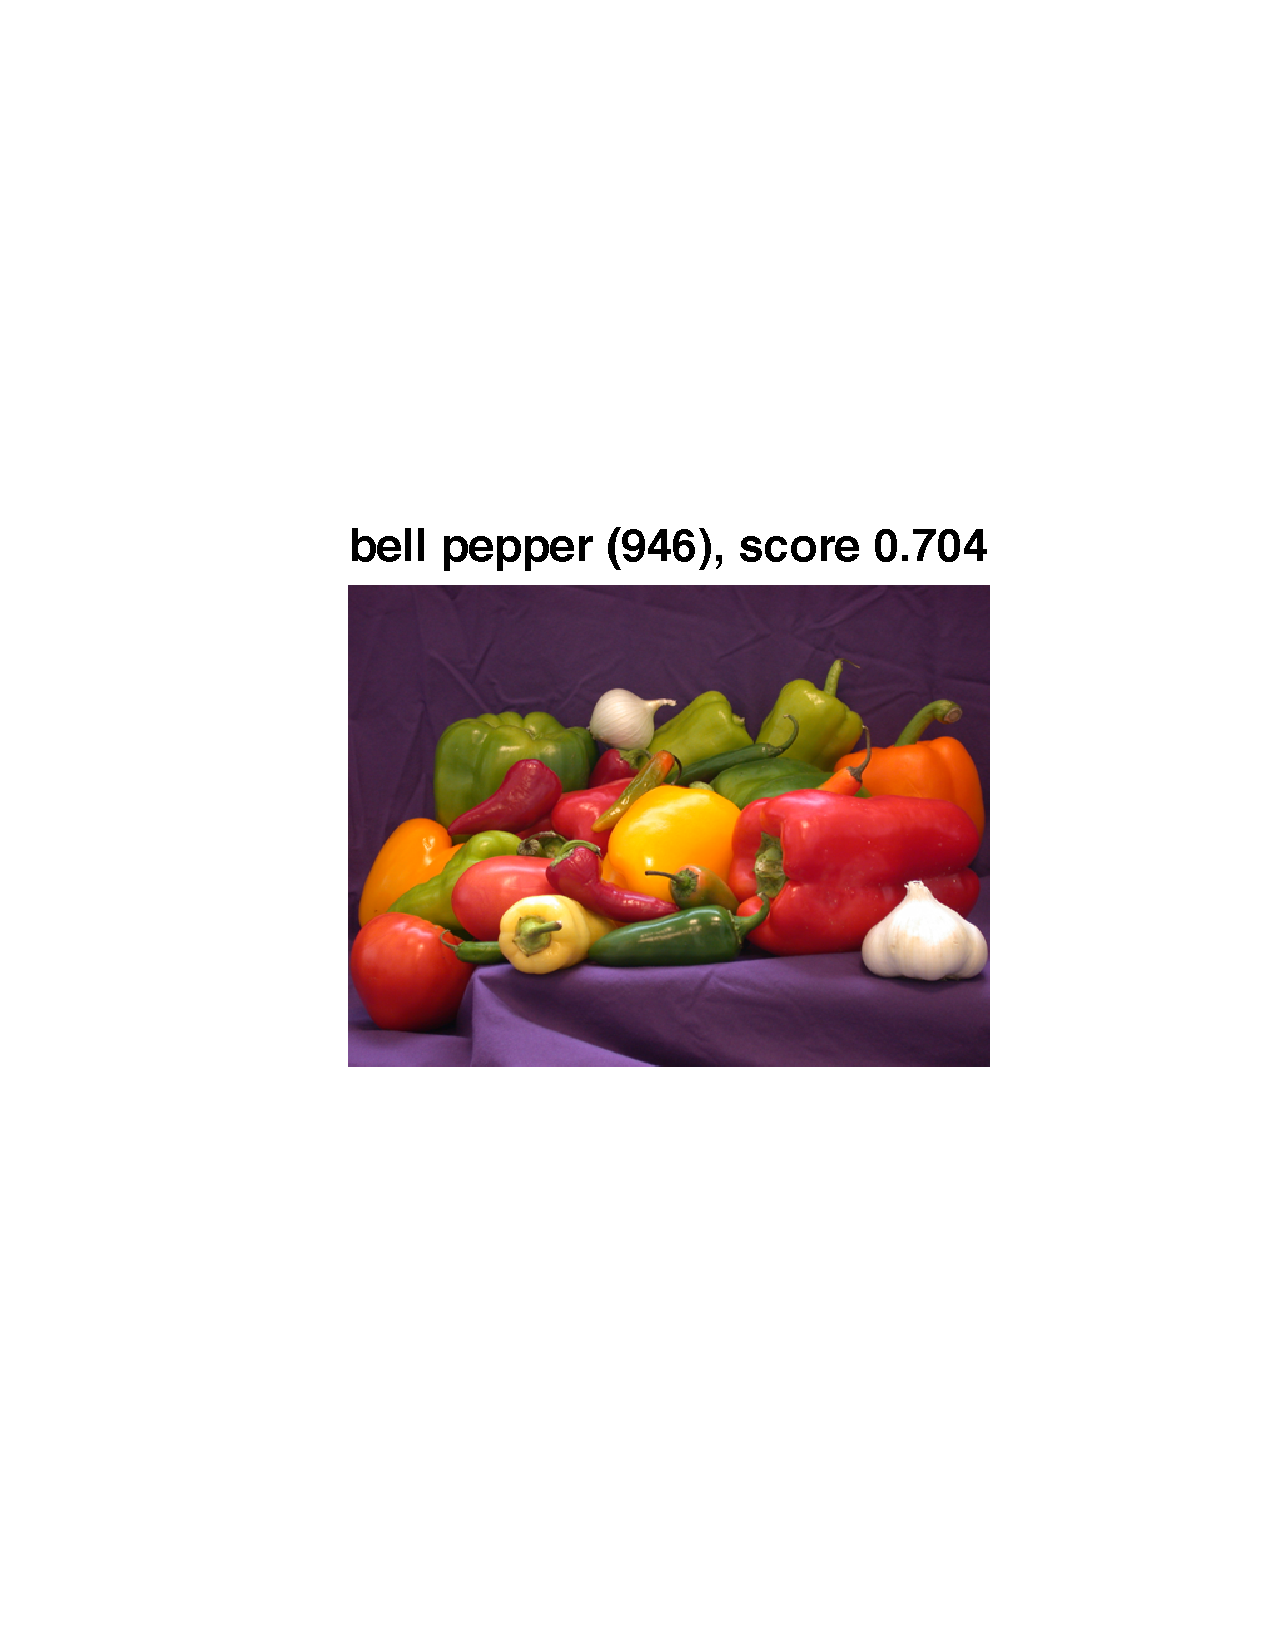
\includegraphics[width=0.5\columnwidth]{figures/pepper}
\hrule
\begin{lstlisting}[escapechar=!]
% install and compile MatConvNet (run once)
untar(['http://www.vlfeat.org/matconvnet/download/' ...
   'matconvnet-1.0-beta12.tar.gz']) ;
cd matconvnet-1.0-beta12
run matlab/vl_compilenn

% download a pre-trained CNN from the web (run once)
urlwrite(...
 'http://www.vlfeat.org/matconvnet/models/imagenet-vgg-f.mat', ...
 'imagenet-vgg-f.mat') ;
  
% setup MatConvNet
run matlab/vl_setupnn

% load the pre-trained CNN
net = load('imagenet-vgg-f.mat') ;

% load and preprocess an image
im = imread('peppers.png') ;
im_ = imresize(single(im), net.meta.normalization.imageSize(1:2)) ;
im_ = im_ - net.meta.normalization.averageImage ;

% run the CNN
res = vl_simplenn(net, im_) ;

% show the classification result
scores = squeeze(gather(res(end).x)) ;
[bestScore, best] = max(scores) ;
figure(1) ; clf ; imagesc(im) ;!
\begin{tikzpicture}[overlay]
\node (x) {};
\node (y) at (7,1) {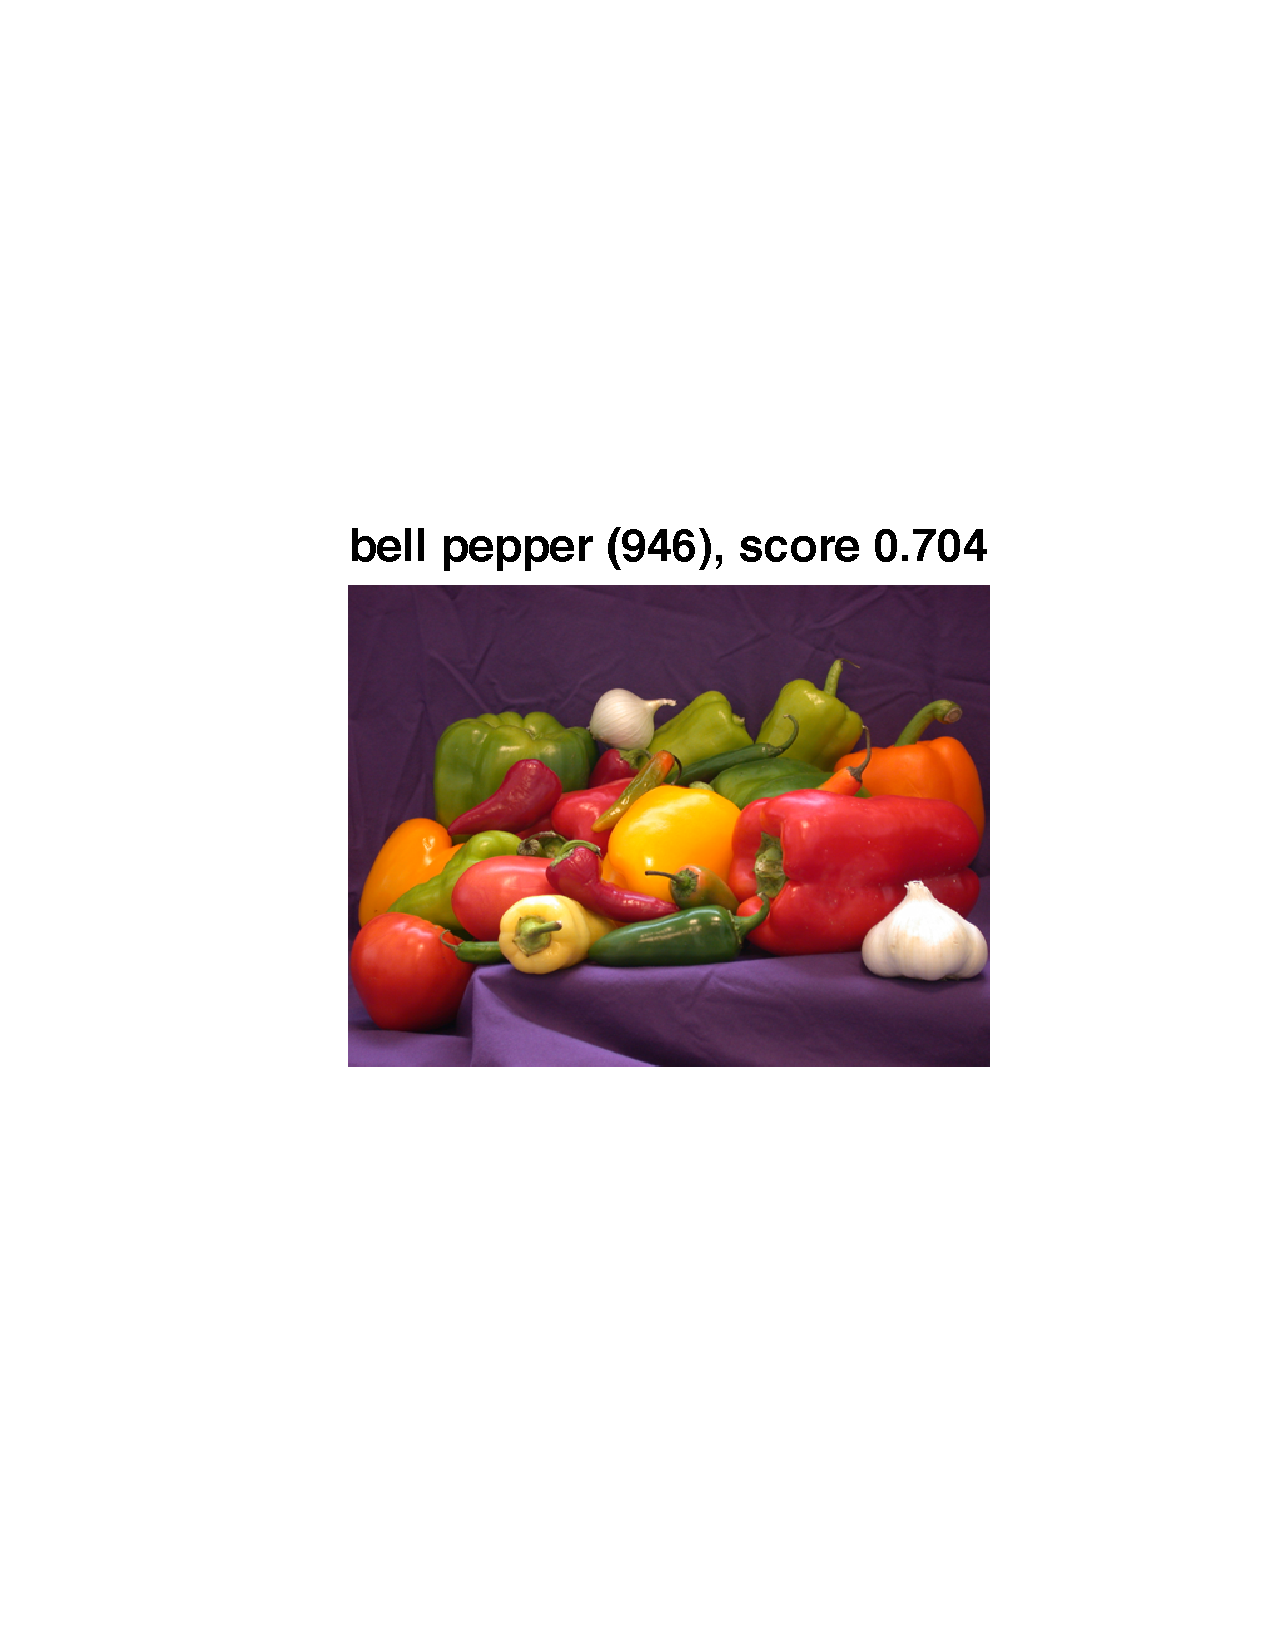
\includegraphics[width=5cm]{figures/pepper}};
\draw [->,thick] (.1,.1) -- (4.5,.1) {};
\end{tikzpicture}!
title(sprintf('%s (%d), score %.3f',...
net.classes.description{best}, best, bestScore)) ;
\end{lstlisting}
\hrule
\caption{A complete example including download, installing, compiling and running  \matconvnet to classify one of  \matlab stock images using a large CNN pre-trained on ImageNet.}
\label{f:demo}
\end{figure}

\matconvnet is simple to install and use. \autoref{f:demo} provides a complete example that classifies an image using a latest-generation deep convolutional neural network. The example includes downloading MatConvNet, compiling the package, downloading a pre-trained CNN model, and evaluating the latter on one of \matlab's stock images.

The key command in this example is !vl_simplenn!, a wrapper that takes as input the CNN !net! and the pre-processed image !im_! and produces as output a structure !res! of results. This particular wrapper can be used to model networks that have a simple structure, namely a \emph{chain} of operations. Examining the code of !vl_simplenn! (!edit vl_simplenn! in \matconvnet) we note that the wrapper transforms the data sequentially, applying a number of \matlab functions as specified by the network configuration. These function, discussed in detail in \autoref{s:blocks}, are called ``building blocks'' and constitute the backbone of \matconvnet. 

%Since blocks are made available as \matlab functions, it is easy for a user to write different wrappers that implement more complex network structures, such as recurrent neural networks. Likewise, it is easy to extend !vl_simplenn! with new building blocks.

While most blocks implement simple operations, what makes them non trivial is their efficiency (\autoref{s:speed}) as well as support for backpropagation (\autoref{s:back}) to allow learning CNNs. Next, we demonstrate how to use one of such building blocks directly. For the sake of the example, consider convolving an image with a bank of linear filters. Start by reading an image in \matlab, say using !im = single(imread('peppers.png'))!, obtaining a $H \times W \times D$ array !im!, where $D=3$ is the number of colour channels in the image. Then create a bank of $K=16$ random filters of size $3 \times 3$ using !f = randn(3,3,3,16,'single')!. Finally, convolve the image with the filters by using the command !y = vl_nnconv(x,f,[])!. This results in an array !y! with $K$ channels, one for each of the $K$ filters in the bank. 

While users are encouraged to make use of the blocks directly to create new architectures, \matlab provides wrappers such as !vl_simplenn! for standard CNN architectures such as AlexNet~\cite{krizhevsky12imagenet} or Network-in-Network~\cite{lin13network}. Furthermore, the library provides numerous examples (in the !examples/! subdirectory), including code to learn a variety models on the MNIST, CIFAR, and ImageNet datasets. All these examples use the !examples/cnn_train! training code, which is an implementation of stochastic gradient descent (\autoref{s:block-list}). While this training code is perfectly serviceable and quite flexible, it remains in the !examples/! subdirectory as it is somewhat problem-specific. Users are welcome to implement their optimisers.

% ------------------------------------------------------------------
\section{\matconvnet at a glance}\label{s:vlnn}
% ------------------------------------------------------------------

\matconvnet has a simple design philosophy. Rather than wrapping CNNs around complex layers of software, it exposes simple functions to compute CNN building blocks, such as linear convolution and ReLU operators, directly as a MATLAB commands. These building blocks are easy to combine into a complete CNNs and can be used to implement sophisticated learning algorithms. While several real-world examples of small and large CNN architectures and training routines are provided, it is always possible to go back to the basics and build your own, using the efficiency of MATLAB in prototyping. Often no C coding is required at all to try a new architectures. As such, \matconvnet is an ideal playground for research in computer vision and CNNs.

\matconvnet contains the following elements:
\begin{itemize}
\item \emph{CNN computational blocks.} A set of optimized routines computing fundamental building blocks of a CNN. For example, a convolution block is implemented by \linebreak !y=vl_nnconv(x,f,b)! where !x! is an image, !f! a filter bank, and !b! a vector of biases (\autoref{s:convolution}). The derivatives are computed as
![dzdx,dzdf,dzdb] = vl_nnconv(x,f,b,dzdy)! where !dzdy! is the derivative of the CNN output w.r.t !y!~(\autoref{s:convolution}). \autoref{s:blocks} describes all the blocks in detail.
\item \emph{CNN wrappers.} \matconvnet provides a simple wrapper, suitably invoked by !vl_simplenn!, that implements a CNN with a linear topology (a chain of blocks). It also provide a much more flexible wrapper supporting networks with arbitrary topologies, encapsulated in the !dagnn.DagNN! MATLAB class.
\item \emph{Example applications.} \matconvnet provides several example of learning CNNs with stochastic gradient descent and CPU or GPU, on MNIST, CIFAR10, and ImageNet data.
\item \emph{Pre-trained models.} \matconvnet provides several state-of-the-art pre-trained CNN models that can be used off-the-shelf, either to classify images or to produce image encodings in the spirit of Caffe or DeCAF.
\end{itemize}

% ------------------------------------------------------------------
\section{Documentation and examples}\label{s:examples}
% ------------------------------------------------------------------

\begin{figure}
\centering
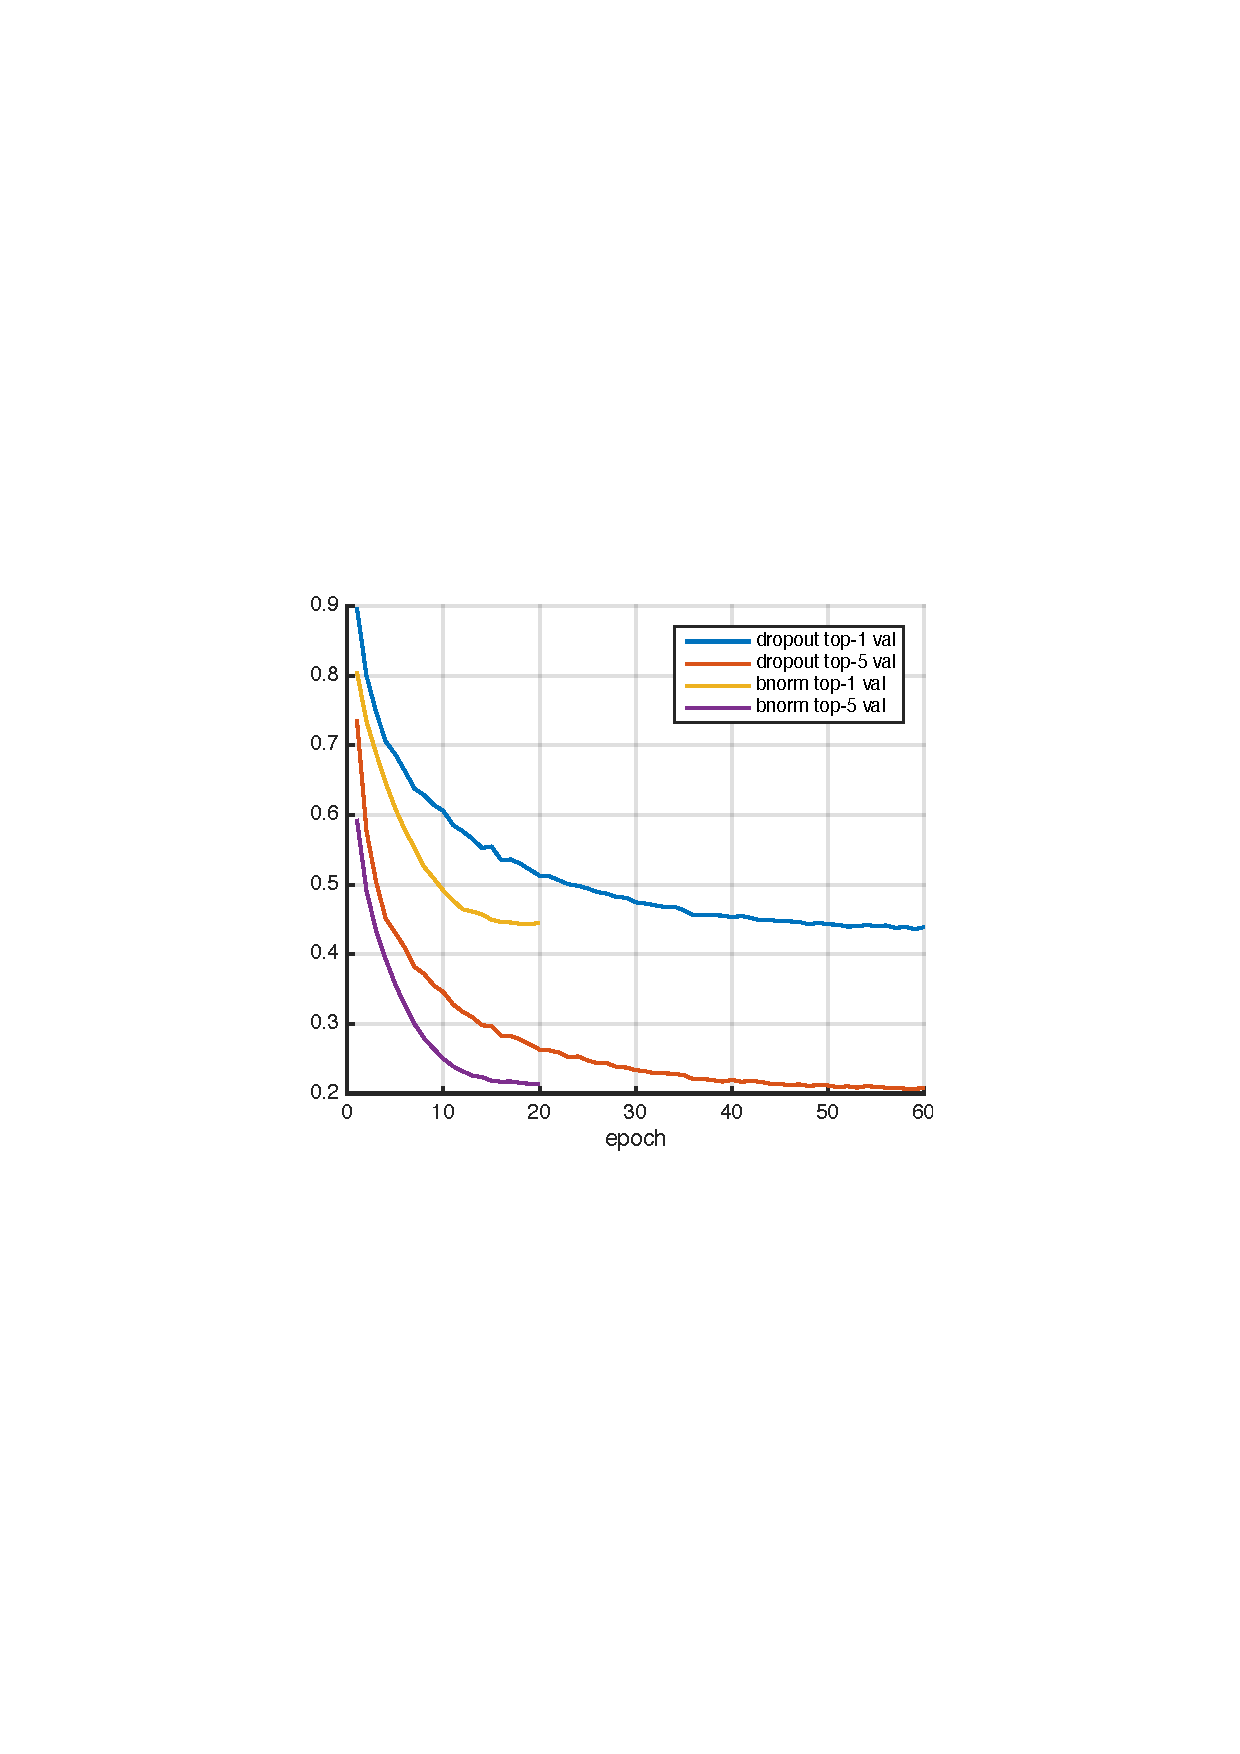
\includegraphics[width=0.65\columnwidth]{figures/imnet}
\vspace{-1em}
\caption{Training AlexNet on ImageNet ILSVRC: dropout vs batch normalisation.}\label{f:imnet}
\end{figure}

There are three main sources of information about \matconvnet. First, the website contains descriptions of all the functions and several examples and tutorials.\footnote{\small See also \url{http://www.robots.ox.ac.uk/~vgg/practicals/cnn/index.html}.} Second, there is a PDF manual containing a great deal of technical details about the toolbox, including detailed mathematical descriptions of the building blocks. Third, \matconvnet ships with several examples (\autoref{s:getting-statrted}).

Most examples are fully self-contained. For example, in order to run the MNIST example, it suffices to point MATLAB to the \matconvnet root directory and type !addpath examples! followed by !cnn_mnist!. Due to the problem size, the ImageNet ILSVRC example requires some more preparation, including downloading and preprocessing the images (using the bundled script !utils/preprocess-imagenet.sh!). Several advanced examples are included as well. For example, \autoref{f:imnet} illustrates the top-1 and top-5 validation errors as a model similar to AlexNet~\cite{krizhevsky12imagenet} is trained using either standard dropout regularisation or the recent \emph{batch normalisation} technique of~\cite{ioffe15batch}. The latter is shown to converge in about one third of the epochs (passes through the training data) required by the former.

The \matconvnet website contains also numerous \emph{pre-trained} models, i.e. large CNNs trained on ImageNet ILSVRC that can be downloaded and used as a starting point for many other problems~\cite{chatfield14return}. These include: AlexNet~\cite{krizhevsky12imagenet}, VGG-S, VGG-M,  VGG-S~\cite{chatfield14return}, and  VGG-VD-16, and VGG-VD-19~\cite{simonyan14very}.  The example code of \autoref{f:demo} shows how one such models can be used in a few lines of MATLAB code.

% ------------------------------------------------------------------
\section{Speed}\label{s:speed}
% ------------------------------------------------------------------

Efficiency is very important for working with CNNs. \matconvnet supports  using NVIDIA GPUs as it includes CUDA implementations of all algorithms (or relies on MATLAB CUDA support). 

 To use the GPU (provided that suitable hardware is available and the toolbox has been compiled with GPU support), one simply converts the arguments to !gpuArrays! in MATLAB, as in !y = vl_nnconv(gpuArray(x), gpuArray(w), [])!. In this manner, switching between CPU and GPU is fully transparent. Note that \matconvnet can also make use of the NVIDIA CuDNN library which significant speed and space benefits.
 
Next we evaluate the performance of \matconvnet when training large architectures on the ImageNet ILSVRC 2012 challenge data~\cite{deng09imagenet}. The test machine is a Dell server with two Intel Xeon CPU E5-2667 v2 clocked at 3.30 GHz (each CPU has eight cores), 256 GB of RAM, and four NVIDIA Titan Black GPUs (only one of which is used unless otherwise noted). Experiments use \matconvnet beta12, CuDNN v2, and MATLAB R2015a. The data is preprocessed to avoid rescaling images on the fly in MATLAB and stored in a RAM disk for faster access. The code uses the !vl_imreadjpeg! command to read large batches of JPEG images from disk in a number of separate threads. The driver !examples/cnn_imagenet.m! is used in all experiments.

 We train the models discussed in \autoref{s:examples} on ImageNet ILSVRC. \autoref{f:speed} reports the training speed as number of images per second processed by stochastic gradient descent. AlexNet trains at about 264 images/s with CuDNN, which is about 40\% faster than the vanilla GPU implementation (using CuBLAS) and more than 10 times faster than using the CPUs. Furthermore, we note that, despite MATLAB overhead, the implementation speed is comparable to Caffe (they report 253 images/s with cuDNN and a Titan -- a slightly slower GPU than the Titan Black used here).  Note also that, as the model grows in size, the size of a SGD batch must be decreased (to fit in the GPU memory), increasing the overhead impact somewhat.
 
 \autoref{f:mgpu} reports the speed on VGG-VD-16, a very large model, using multiple GPUs. In this case, the batch size is set to 264 images. These are further divided in sub-batches of 22 images each to fit in the GPU memory; the latter are then distributed among one to four GPUs on the same machine. While there is a substantial communication overhead, training speed increases from 20 images/s to 45. Addressing this overhead is one of the medium term goals of the library.

\begin{table}
\centering
\begin{tabular}{|lc|ccc|}
  \hline
  model     & batch sz. & CPU  & GPU   & CuDNN \\
  \hline
  AlexNet   & 256       & 22.1 & 192.4 & 264.1 \\
  VGG-F     & 256       & 21.4 & 211.4 & 289.7 \\
  VGG-M     & 128       & 7.8  & 116.5 & 136.6 \\
  VGG-S     & 128       & 7.4  & 96.2  & 110.1 \\
  VGG-VD-16 & 24        & 1.7  & 18.4  & 20.0  \\
  VGG-VD-19 & 24        & 1.5  & 15.7  & 16.5  \\
  \hline
\end{tabular}
\caption{ImageNet training speed (images/s).}
\label{f:speed}
\end{table}

\begin{table}
\centering
\begin{tabular}{|c|cccc|}
  \hline
  num GPUs     & 1  & 2 & 3 & 4 \\
  \hline
  VGG-VD-16 speed & 20.0 & 22.20 & 38.18 & 44.8 \\
  \hline
\end{tabular}
\caption{Multiple GPU speed (images/s).}
\label{f:mgpu}
\end{table}


% --------------------------------------------------------------------
\section{Future}\label{s:future}
% --------------------------------------------------------------------

\matconvnet is a novel framework for experimenting with deep convolutional networks that is deeply integrated in MATLAB and allows easy experimentation with novel ideas.  \matconvnet is already sufficient for advanced research in deep learning; despite being introduced less than a year ago, it is already citied 24 times in arXiv papers, and has been used in several papers published at the recent CVPR 2015 conference. 

As CNNs are a rapidly moving target, \matconvnet is developing fast. So far there have been  12 ad-interim releases incrementally adding new features to the toolbox. Several new features, including support for DAGs, will be included in the upcoming releases starting in August 2015.  The goal is to ensure that \matconvnet will stay current for the next several years of research in deep learning.

% ------------------------------------------------------------------
\section{Acknowledgments}\label{s:ack}
% ------------------------------------------------------------------

\matconvnet is a community project, and as such acknowledgments got to all contributors. We kindly thank NVIDIA supporting this project by providing us with top-of-the-line GPUs and MathWorks for ongoing discussion on how to improve the library. 

The implementation of several CNN computations in this library are inspired by the Caffe library~\cite{jia13caffe} (however, Caffe is \emph{not} a dependency). Several of the example networks have been trained by Karen Simonyan as part of~\cite{chatfield14return} and~\cite{simonyan15very}.
